\documentclass[10pt,a4paper]{amsart}
\usepackage[margin=19mm]{geometry}
\usepackage{amsmath,amssymb,mathtools}
\usepackage[scr=rsfs,cal=euler]{mathalfa}
\usepackage{xfrac}
\usepackage[unicode,hidelinks,bookmarks=false]{hyperref}
\newcommand{\ie}{i.e.\ }
\newcommand{\cf}{cf.\ }
\newcommand{\resp}{respectively\ }
\newcommand{\Subsection}{\subsection}
\providecommand{\nobreakdash}{\nobreak\hbox{-}}
\setlength{\emergencystretch}{2em}
\multlinegap0pt
\usepackage{tikz}
\usepackage{amssymb}
\usepackage{mathtools}
\usepackage[shortlabels]{enumitem}
\newtheorem{lemma}{Lemma}
\title{Classification of Certain C*-Algebras Generated by Two Partitions of Unity}
\author{Bj\"orn Sch\"afer}
\date{Source: arXiv:2509.01309v1 (CC BY 4.0)}
\begin{document}
\maketitle

\noindent\emph{Source and licence.} Classification of Certain C*-Algebras Generated by Two Partitions of Unity. Version arXiv:2509.01309v1 (CC BY 4.0), distributed by arXiv under the Creative Commons Attribution 4.0 International licence, http://creativecommons.org/licenses/by/4.0/, as recorded in the arXiv licence metadata for this exact version and shown on the abstract page https://arxiv.org/abs/2509.01309v1. Full licence notice: \texttt{licenses/arxiv-2509.01309-CC-BY-4.0.txt}.\par\smallskip

\noindent\textit{Editorial scope.} Counted unit: the article's lemma class::lemma:phi\_is\_invertible (source0.tex lines 1452--1455). The article's complete original proof of it is delivered with it (source0.tex lines 1457--1610, one \texttt{proof} environment of 154 lines). No mathematics is written, repaired or re-derived: the statement and the proof are the article's own lines, in the article's own notation, and no retained line is substituted or re-flowed.  Retained uncounted as the source-local context the proof needs: lines 233--236; lines 263--275; lines 1128--1131.  Nothing was omitted from any retained span, so the package carries no omission record.  No retained line contains a citation, so the wrapper carries no bibliography and no bibliography entry.  The retained lines contain the article's own diagram code, which the wrapper typesets with the standard tikz packages; no image file is delivered and the package declares no asset dependency.  Editorial formatting only, in addition: an AMS \texttt{amsart} preamble that restates the article's own declarations and macros used by the retained lines, namely the environments \texttt{lemma} on separate counters, together with the standard packages those lines need.  The retained environments print in this document as Lemma 1 in order of appearance, whereas the article prints the same items with the numbering of its own full document.  The complete native source of the article as distributed in the arXiv e-print for this exact version is bundled unchanged as \texttt{sources/184234/source0.tex}.
    \begin{align}
        \sum_{u \in U} p_u &= 1 = \sum_{v \in V} p_v,        \tag{GP1} \label{bga::eq:partition_relation} \\
        p_u p_v &= 0 \; \text{ if } \{u, v\} \not \in E.     \tag{GP2} \label{bga::eq:orthogonality_relation}
    \end{align}

\begin{lemma}
    \label{bga::lemma:nontrivial_p_x2 p_y p_x2_and_K22_subgraph}
    Let $G = (U, V, E)$ be a bipartite graph, and let $x_1, x_2, y \in U \cup V$ be three distinct vertices. Then 
    \begin{align*}
        p_{x_1} p_y p_{x_2} \neq 0
        \quad \implies \quad 
        \{y\} \subsetneq \mathcal{N}(x_1) \cap \mathcal{N}(x_2).
    \end{align*}
    In particular, in this case there must be a fourth vertex $y^\prime$ such that 
    $$
    G(x_1, x_2, y, y^\prime) \cong K_{2,2}.
    $$
\end{lemma}

    \begin{align}
        \label{reps::eq:f_preserves_adjacency}
        e_i \text{ and } e_j \text{ are adjacent} \quad\Leftrightarrow\quad f(e_i) \text{ and } f(e_j) \text{ are adjacent}.
    \end{align}

\begin{lemma} 
    \label{class::lemma:phi_is_invertible}
    One has $\varphi_{f^{-1}} \circ \varphi_f = \mathrm{id}_{C^\ast(G)}$.
\end{lemma}

\begin{proof}
    It suffices to show 
    \begin{align*}
        \varphi_{f^{-1}}(\varphi_f(p_x)) = p_x,
    \end{align*}
    for all $x \in U \cup V$. Indeed, we only prove this for $x \in U$ because the case $x \in V$ is analogous. Thus, let $u \in U$ be fixed.
    The definitions of $\varphi_{f^{-1}}$ and $\varphi_f$, respectively, yield 
    \begin{align*}
        \varphi_{f^{-1}}(\varphi_f(p_u))
            &= \varphi_{f^{-1}}\left( \sum_{\{u^\prime, v^\prime\} \in I(u)} \hat{p}_{u^\prime} \hat{p}_{v^\prime} \right) \\
            &= \sum_{\{u^\prime, v^\prime\} \in I(u)} \left( \sum_{\{u_1, v_1\} \in J(u^\prime)} p_{u_1} p_{v_1} \right) \left( \sum_{\{u_2, v_2\} \in J(v^\prime)} p_{u_2} p_{v_2} \right).
    \end{align*}
    Using $\varphi_{f^{-1}}(\hat{p}_{u^\prime}) = \left(\varphi_{f^{-1}}(\hat{p}_{u^\prime})\right)^\ast = \sum_{\{u_1, v_1\} \in J(u^\prime)} p_{v_1} p_{u_1}$ together with \eqref{bga::eq:orthogonality_relation} we can continue the computation as follows:
    \begin{align*}
        \varphi_{f^{-1}}(\varphi_f(p_u))
            &= \sum_{\{u^\prime, v^\prime\} \in I(u)} \left( \sum_{\{u_1, v_1\} \in J(u^\prime)}  p_{v_1} p_{u_1}\right) \left( \sum_{\{u_2, v_2\} \in J(v^\prime)} p_{u_2} p_{v_2} \right) \\
            &= \sum_{\{u^\prime, v^\prime\} \in I(u)} \left( \sum_{\{u_1, v_1\} \in J(u^\prime), \{u_1, v_2\} \in J(v^\prime)} p_{v_1} p_{u_1} p_{v_2} \right).
    \end{align*}
    We claim
    \begin{align*} 
        &\left\{(v_1, u_1, v_2) \left| \;
            \begin{aligned}
                &\{u_1, v_1\} \in J(u^\prime) \\
                &\{u_1, v_2\} \in J(v^\prime)
            \end{aligned} \;
                \text{ for some } \{u^\prime, v^\prime\} \in I(u)
                \text{ with } p_{v_1} p_{u_1} p_{v_2} \neq 0 
            \right. \right\} \\
        &=\{(v_1, u, v_2): V \ni v_1 \sim u \sim v_2 \in V \text{ with } p_{v_1} p_u p_{v_2} \neq 0 \},
    \end{align*}
    where $u$ remains the fixed vertex from above.
    First, assume that $(v_1, u, v_2)$ is in the set on the right-hand side, i.e. 
    $$ V \ni v_1 \sim u \sim v_2 \in V \quad \text{with} \quad p_{v_1} p_u p_{v_2} \neq 0. $$ 
    There are two possibilities. If $v_1 = v_2$, then setting $\{u^\prime, v^\prime\} := f(\{u, v_1\})$ one easily verifies $\{u, v_1\} \in J(u^\prime) \cap J(v^\prime)$ while $\{u^\prime, v^\prime\} \in I(u)$. Thus, the triple $(v_1, u, v_2)$ is in the set on the left-hand side.
    
    Next, assume $v_1 \neq v_2$. As $p_{v_1} p_u p_{v_2}$ is non-zero, Lemma \ref{bga::lemma:nontrivial_p_x2 p_y p_x2_and_K22_subgraph} yields some vertex $u_2 \in U$ such that the graph from Figure \ref{class::fig:G(u, v_1, v_2, u_2)} is a subgraph of $G$.
%
    \begin{figure}[htb]
        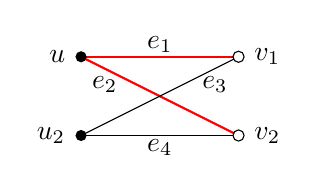
\begin{tikzpicture}
            % horizontal edges
            \draw[thick, color=red] (-1,2) -- (1, 2);
            \draw (-1,1) -- (1, 1);
            % diagonal edges
            \draw[thick, color=red] (-1,2) -- (1, 1);
            \draw (-1,1) -- (1, 2);
            % labels for horizontal edges
            \node[label=90:$e_1$] at (0, 1.8) {};
            \node[label=-90:$e_4$] at (0, 1.2) {};
            % labels for diagonal edges
            \node[label=90:$e_2$] at (-.7, 1.3) {};
            \node[label=90:$e_3$] at (.7, 1.3) {};
            % left vertices
            \node[label=180:$u$, fill=black, circle, inner sep=.05cm] at (-1, 2) {};
            \node[label=180:$u_2$, fill=black, circle, inner sep=.05cm] at (-1, 1) {};
            % right vertices
            \node[label=0:$v_1$, fill=white, draw=black, circle, inner sep=.05cm] at (1, 2) {};
            \node[label=0:$v_2$, fill=white, draw=black, circle, inner sep=.05cm] at (1, 1) {};
        \end{tikzpicture}
        \caption{The subgraph $G(u, v_1, v_2, u_2)$}
        \label{class::fig:G(u, v_1, v_2, u_2)}
    \end{figure}
% 
    As $e_1$ and $e_2$ are adjacent in $G(e_1, e_2, e_3, e_4)$, by Property \eqref{reps::eq:f_preserves_adjacency} the same holds in $G^\prime(f(e_1), f(e_2), f(e_3), f(e_4))$. Thus, the subgraph $G^\prime(f(e_1), f(e_2))$ must take one of the two forms shown in Figure \ref{class::fig:G(f(e_1), f(e_2))}.
    \begin{figure}[htb]
        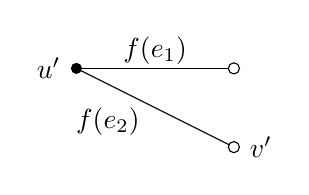
\begin{tikzpicture}
            % horizontal edges
            \draw (-1,2) -- (1, 2);
            % diagonal edges
            \draw (-1,2) -- (1, 1);
            % labels for horizontal edges
            \node[label=90:$f(e_1)$] at (0, 1.8) {};
            % labels for diagonal edges
            \node[label=90:$f(e_2)$] at (-.6, .9) {};
            % left vertices
            \node[label=180:$u^\prime$, fill=black, circle, inner sep=.05cm] at (-1, 2) {};
            % right vertices
            \node[fill=white, draw=black, circle, inner sep=.05cm] at (1, 2) {};
            \node[label=0:$v^\prime$, fill=white, draw=black, circle, inner sep=.05cm] at (1, 1) {};
        \end{tikzpicture}
        $\quad$
        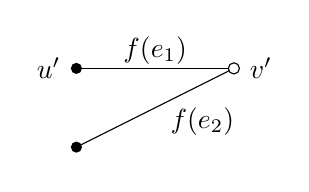
\begin{tikzpicture}
            % horizontal edges
            \draw (-1,2) -- (1, 2);
            % diagonal edges
            \draw (-1,1) -- (1, 2);
            % labels for horizontal edges
            \node[label=90:$f(e_1)$] at (0, 1.8) {};
            % labels for diagonal edges
            \node[label=90:$f(e_2)$] at (.6, .9) {};
            % left vertices
            \node[label=180:$u^\prime$, fill=black, circle, inner sep=.05cm] at (-1, 2) {};
            \node[ fill=black, circle, inner sep=.05cm] at (-1, 1) {};
            % right vertices
            \node[label=0:$v^\prime$, fill=white, draw=black, circle, inner sep=.05cm] at (1, 2) {};
        \end{tikzpicture}
        \caption{The two possible forms of the subgraph $G^\prime(f(e_1), f(e_2))$}
        \label{class::fig:G(f(e_1), f(e_2))}
    \end{figure} 
    Choosing the vertices $u^\prime \in f(e_1)$ and $v^\prime \in f(e_2)$ as in the figure one easily checks $\{u^\prime, v^\prime\} \in I(u)$ as well as $e_1 = \{u, v_1\} \in J(u^\prime)$ and $e_2 = \{u, v_2\} \in J(v^\prime)$. Thus, the triple $(v_1, u, v_2)$ is in the set on the left-hand side, and this concludes the proof of the inclusion $(\mathrm{lhs}) \supseteq (\mathrm{rhs})$. 

    For the other inclusion, assume that $(v_1, u_1, v_2)$ is in the set on the left-hand side, i.e.
    \begin{align*}
            \begin{aligned}
                &\{u_1, v_1\} \in J(u^\prime) \\
                &\{u_1, v_2\} \in J(v^\prime)
            \end{aligned} \;
                \text{ for some } \{u^\prime, v^\prime\} \in I(u)
                \text{ with } p_{v_1} p_{u_1} p_{v_2} \neq 0.
    \end{align*}
    It suffices to show $u_1 = u$ since $p_{v_1} p_{u_1} p_{v_2} \neq 0$ implies $v_1 \sim u_1 \sim v_2$ (using \eqref{bga::eq:orthogonality_relation}) and thus the triple $(v_1, u_1, v_2)$ is in the set on the right-hand side.

    If $v_1 = v_2$, then we obtain immediately $f(\{u_1, v_1\}) = \{u^\prime, v^\prime\} \in I(u)$ and this yields $u^\prime = u$. 

    Next, assume $v_1 \neq v_2$. In view of Lemma \ref{bga::lemma:nontrivial_p_x2 p_y p_x2_and_K22_subgraph} there exists some $u_2 \in U$ such that the graph from Figure \ref{class::fig:G(u_1, v_1, v_2, u_2)} is a subgraph of $G$. %following is a subgraph of $G$.
%
    \begin{figure}[htb]
        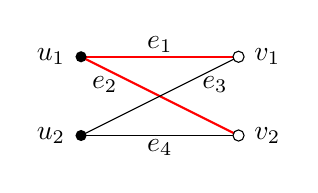
\begin{tikzpicture}
            % horizontal edges
            \draw[thick, color=red] (-1,2) -- (1, 2);
            \draw (-1,1) -- (1, 1);
            % diagonal edges
            \draw[thick, color=red] (-1,2) -- (1, 1);
            \draw (-1,1) -- (1, 2);
            % labels for horizontal edges
            \node[label=90:$e_1$] at (0, 1.8) {};
            \node[label=-90:$e_4$] at (0, 1.2) {};
            % labels for diagonal edges
            \node[label=90:$e_2$] at (-.7, 1.3) {};
            \node[label=90:$e_3$] at (.7, 1.3) {};
            % left vertices
            \node[label=180:$u_1$, fill=black, circle, inner sep=.05cm] at (-1, 2) {};
            \node[label=180:$u_2$, fill=black, circle, inner sep=.05cm] at (-1, 1) {};
            % right vertices
            \node[label=0:$v_1$, fill=white, draw=black, circle, inner sep=.05cm] at (1, 2) {};
            \node[label=0:$v_2$, fill=white, draw=black, circle, inner sep=.05cm] at (1, 1) {};
        \end{tikzpicture}
        \caption{The graph $G(u_1, v_1, v_2, u_2)$}
        \label{class::fig:G(u_1, v_1, v_2, u_2)}
    \end{figure}
%  
    where $e_1 \in J(u^\prime)\; ( \Leftrightarrow u^\prime \in f(e_1))$, and $e_2 \in J(v^\prime)\; ( \Leftrightarrow v^\prime \in f(e_2))$.
    Again by Property \eqref{reps::eq:f_preserves_adjacency} the subgraph $G^\prime(f(e_1), f(e_2))$ must take one of the two forms shown in Figure \ref{class::fig:G(f(e_1), f(e_2))}. The vertices $u^\prime$ and $v^\prime$ must be as depicted since $e_1 \in J(u^\prime)$ and $e_2 \in J(v^\prime)$. Now, one sees that either $f(e_1) = \{u^\prime, v^\prime\}$ or $f(e_2) = \{u^\prime, v^\prime\}$. Then the assumption $\{u^\prime, v^\prime\} \in I(u)$ implies $f(e_1) \in I(u)$ or $f(e_2) \in I(u)$. In any event, it follows that $u_1 = u$.

    Putting everything together we obtain
    \begin{align*}
        \varphi_{f^{-1}}(\varphi_f(p_u))
            &= \sum_{\{u^\prime, v^\prime\} \in I(u)} \left( \sum_{\{u_1, v_1\} \in J(u^\prime), \{u_1, v_2\} \in J(v^\prime)} p_{v_1} p_{u_1} p_{v_2} \right) \\
            &= \sum_{V \ni v_1 \sim u \sim v_2 \in V} p_{v_1} p_u p_{v_2} \\
            &= \sum_{v_1, v_2 \in V} p_{v_1} p_u p_{v_2} \\
            &= \left( \sum_{v_1 \in V} p_{v_1} \right) p_u \left( \sum_{v_2 \in V} p_{v_2} \right) \\
            &= p_u,
    \end{align*}
    where we use the claim for the step from the first to the second line. The last two equalities follows from \eqref{bga::eq:orthogonality_relation} and \eqref{bga::eq:partition_relation}, respectively.
\end{proof}

\end{document}
